\documentclass{article}
\usepackage{graphicx} 
\usepackage[utf8]{inputenc}



\begin{document}
  \begin{titlepage}
  \title{How does the time it takes a ball to roll down a slope depend on the distance it travels?}
  \maketitle
  \author{Authors: Jason Wells, Kevin Qiao, Stephen Okita and Terri Tai}
  \date{October 26th. 2021}
  \centering
  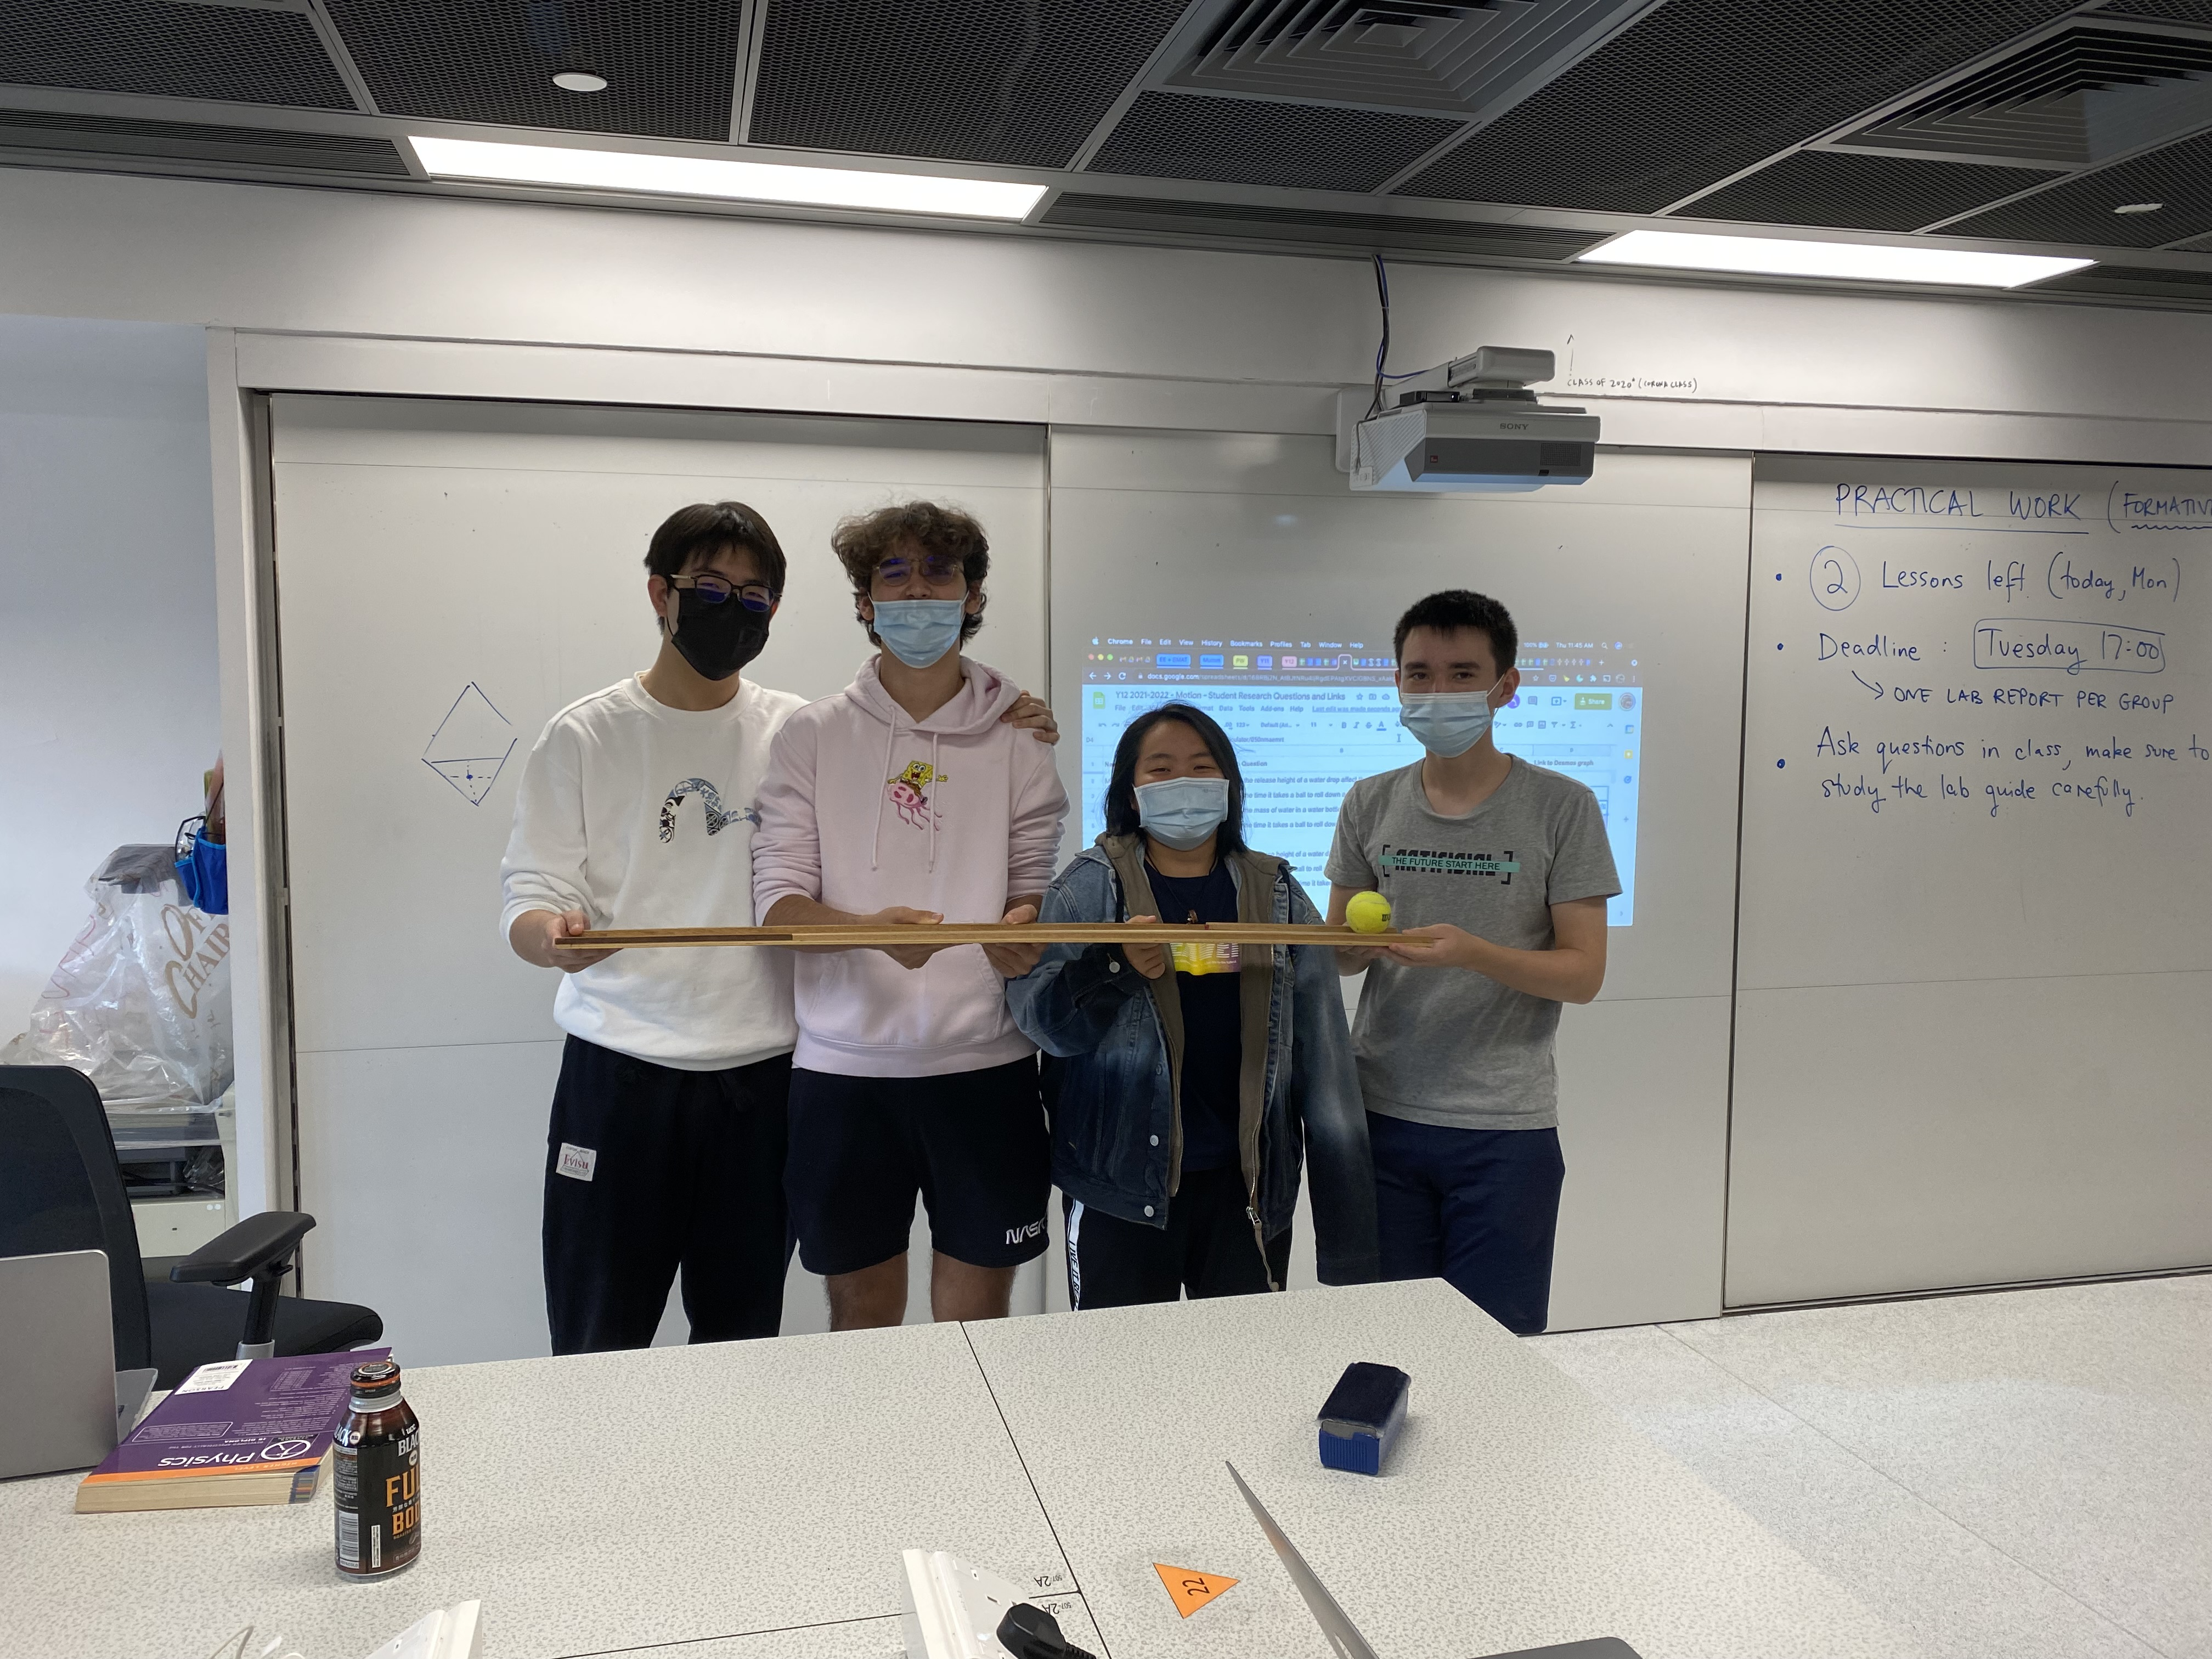
\includegraphics[width=14cm]{theTeam.jpg} % also works with logo.pdf
  \end{titlepage}

\tableofcontents

\section{Introduction}
​   \[s = ut\]
\begin{abstract}
This is a document to help my learning and document my philosophical and mathematical ideas. What is the formating of this i
\end{abstract}

\begin{center}
What is the purpose of a rubber duck, is humanity doomed by excesses. If one was to represent how fuked humanity is we could model it with: 
\end{center}
\[ y = \sqrt{\frac{2x}{-9.8(\sin(5.17))-0.14\cos(5.17)}}\]

\end{document}\